\documentclass{article}
% generated by Madoko, version 1.1.3
%mdk-data-line={1}


\usepackage[heading-base={2},section-num={False},bib-label={hide},fontspec={True}]{madoko2}


\begin{document}



%mdk-data-line={4}
\mdxtitleblockstart{}
%mdk-data-line={4}
\mdxtitle{\mdline{4}Angel调研及试用报告}%mdk
\mdxauthorstart{}
%mdk-data-line={9}
\mdxauthorname{\mdline{9}ryanyycao(曹洋毓)}%mdk
\mdxauthorend\mdtitleauthorrunning{}{}\mdxtitleblockend%mdk

%mdk-data-line={6}
\section{\mdline{6}1.\hspace*{0.5em}\mdline{6}综述}\label{section}%mdk%mdk

%mdk-data-line={8}
\noindent\mdline{8}Angel是一个基于参数服务器的高性能分布式机器学习平台,核心设计理念围绕机器学习模型,将高维度的大模型合理切分到多个参数服务器节点。
Angel的主要核心抽象是PSModel,它将对分布于多台PS Server上的远程模型操作透明化,通过PSModel,用户可以方便的进行模型的更新,
自定义函数计算,以及同步控制,从而实现各种高效的机器学习算法。Angel基于Java和Scala进行开发,可以使用Yarn直接调度运行,支持
Spark on Angel%mdk

%mdk-data-line={13}
\section{\mdline{13}2.\hspace*{0.5em}\mdline{13}架构设计}\label{section}%mdk%mdk

%mdk-data-line={14}
\noindent\mdline{14}Angel中的各种角色:%mdk

%mdk-data-line={16}
\begin{mddefinitions}%mdk

\mddefterm{\noindent{\bfseries Client}}%mdk

%mdk-data-line={16}
\begin{mdbmarginx}{}{}{}{1.5em}%mdk
\begin{mddefdata}%mdk
\mdline{16}控制任务运行,启动和停止Angel任务,加载和存储模型,启动具体计算过程和获取任务运行状态等
%mdk
\end{mddefdata}%mdk
\end{mdbmarginx}%mdk

\mddefterm{\noindent{\bfseries Master}}%mdk

%mdk-data-line={18}
\begin{mdbmarginx}{}{}{}{1.5em}%mdk
\begin{mddefdata}%mdk
\mdline{18}原始计算数据以及参数矩阵的分片和分发,申请Worker和ParameterServer所需的计算资源,协调,管理和监控Worker以及ParameterServer
%mdk
\end{mddefdata}%mdk
\end{mdbmarginx}%mdk

\mddefterm{\noindent{\bfseries Parameter Server}}%mdk

%mdk-data-line={20}
\begin{mdbmarginx}{}{}{}{1.5em}%mdk
\begin{mddefdata}%mdk
\mdline{20}负责存储和更新参数
%mdk
\end{mddefdata}%mdk
\end{mdbmarginx}%mdk

\mddefterm{\noindent{\bfseries Worker}}%mdk

%mdk-data-line={22}
\begin{mdbmarginx}{}{}{}{1.5em}%mdk
\begin{mddefdata}%mdk
\mdline{22}负责具体的模型训练或者结果预测,一个计算任务往往包含许多个Worker实例,每个Worker实例负责使用一部分训练数据进行训练%mdk
\end{mddefdata}%mdk
\end{mdbmarginx}%mdk
%mdk
\end{mddefinitions}%mdk

%mdk-data-line={24}
\noindent\mdline{24}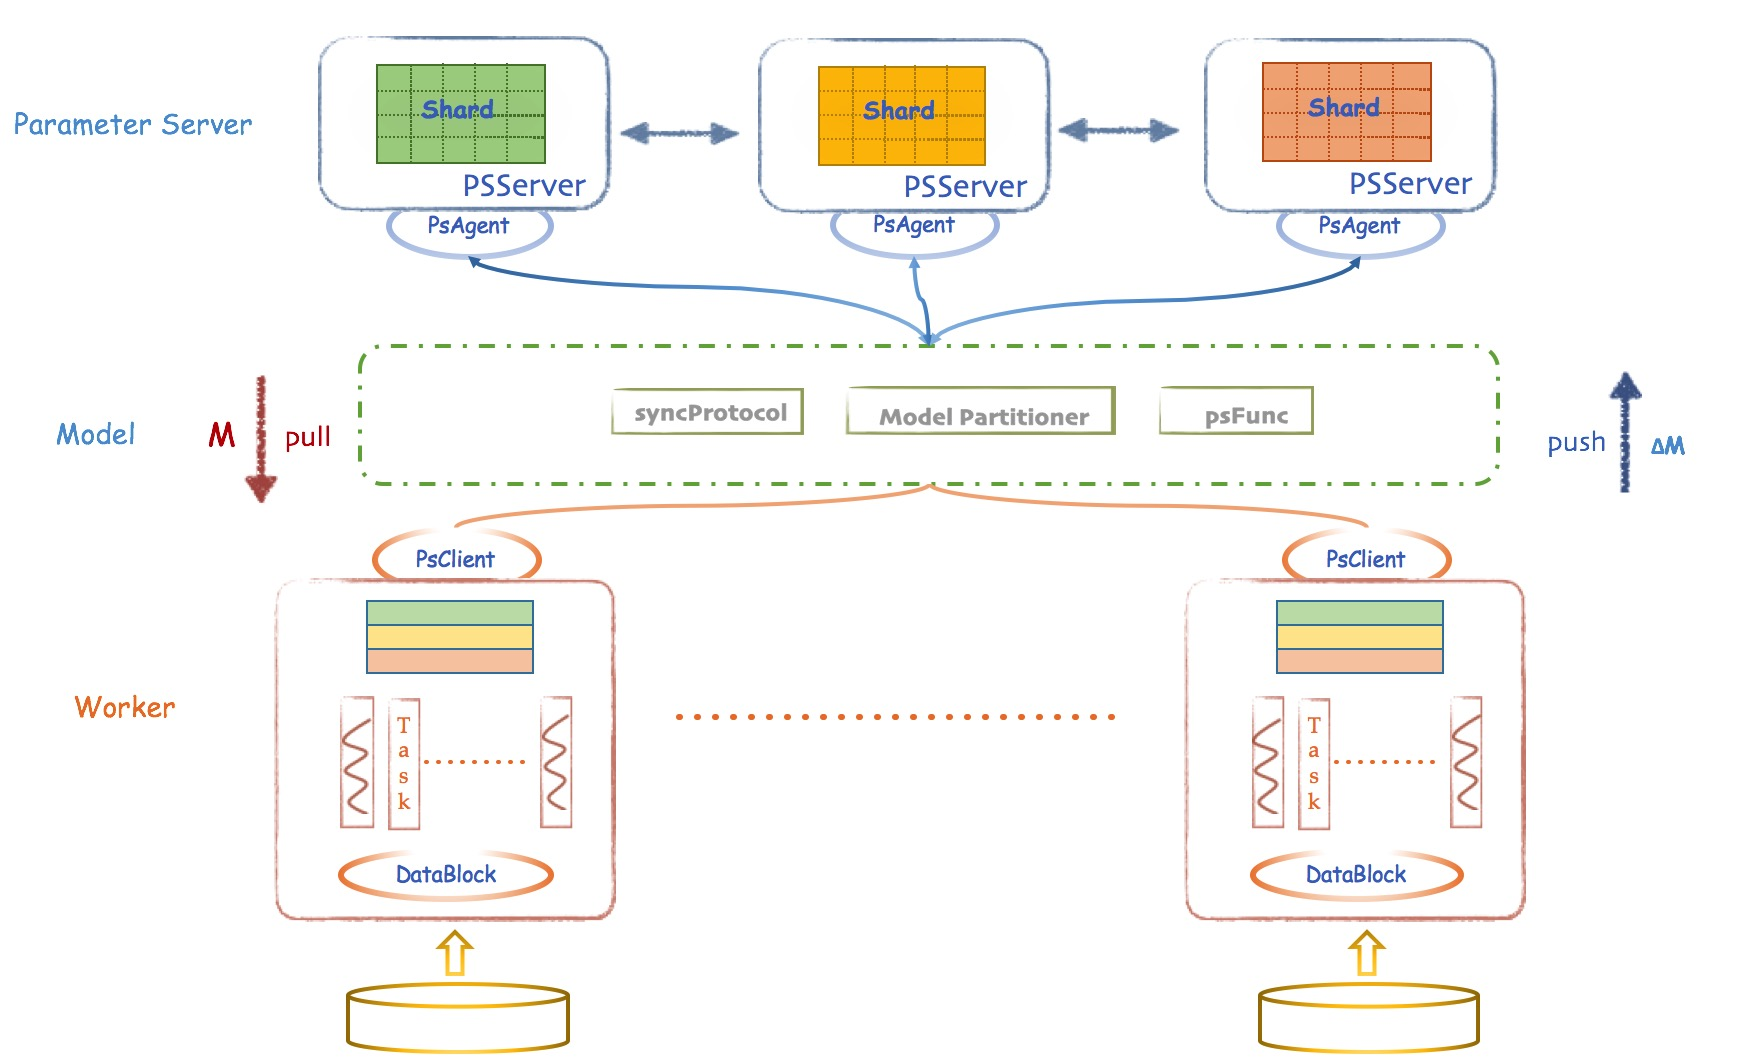
\includegraphics[keepaspectratio=true,width=\dimmin{}{\dimwidth{0.90}}]{images/angel_architecture_1}{}\mdline{24}
\mdline{25} \mdline{25}%mdk

%mdk-data-line={28}
\noindent\mdline{28}Angel中的核心抽象:%mdk

%mdk-data-line={30}
\begin{mddefinitions}%mdk

\mddefterm{\noindent{\bfseries PSModel(远程模型)}}%mdk

%mdk-data-line={30}
\begin{mdbmarginx}{}{}{}{1.5em}%mdk
\begin{mddefdata}%mdk
\mdline{30}PSModel是一个远程模型的概念,对于Client来说,它是一个类似模型代理的类。通过它你可以在每个Worker上,像操作本地对象一样去操作一个模型,而实际上你操作的是一个均匀切分在远程多个PSServer上的分布式模型切片,而且所有的操作都是透明并发的
%mdk
\end{mddefdata}%mdk
\end{mdbmarginx}%mdk

\mddefterm{\noindent{\bfseries MLModel(模型集)}}%mdk

%mdk-data-line={32}
\begin{mdbmarginx}{}{}{}{1.5em}%mdk
\begin{mddefdata}%mdk
\mdline{32}由一系列的PSModel(远程模型)构成,对这些模型进行统一操作%mdk
\end{mddefdata}%mdk
\end{mdbmarginx}%mdk
%mdk
\end{mddefinitions}%mdk

%mdk-data-line={35}
\section{\mdline{35}3.\hspace*{0.5em}\mdline{35}高级特性}\label{section}%mdk%mdk

%mdk-data-line={37}
\begin{mddefinitions}%mdk

\mddefterm{\noindent{\bfseries多种参数同步协议(通过向量时钟实现)}}%mdk

%mdk-data-line={37}
\begin{mdbmarginx}{}{}{}{1.5em}%mdk
\begin{mddefdata}%mdk

%mdk-data-line={37}
\mdline{37}BSP:在每一轮迭代中都需要等待所有的Task计算完成%mdk
%mdk
\end{mddefdata}%mdk
\end{mdbmarginx}%mdk

%mdk-data-line={39}
\begin{mdbmarginx}{}{}{}{1.5em}%mdk
\begin{mddefdata}%mdk

%mdk-data-line={39}
\mdline{39}SSP:允许一定程度的Task进度不一致,但这个不一致有一个上限%mdk
%mdk
\end{mddefdata}%mdk
\end{mdbmarginx}%mdk

%mdk-data-line={40}
\begin{mdbmarginx}{}{}{}{1.5em}%mdk
\begin{mddefdata}%mdk

%mdk-data-line={40}
\mdline{40}ASP:Task之间完全不用相互等待,先完成的Task,继续下一轮的训练%mdk
%mdk
\end{mddefdata}%mdk
\end{mdbmarginx}%mdk

\mddefterm{\noindent{\bfseries ps function(psf)}}%mdk

%mdk-data-line={42}
\begin{mdbmarginx}{}{}{}{1.5em}%mdk
\begin{mddefdata}%mdk

%mdk-data-line={42}
\mdline{42}通过继承Angel提供的psf函数接口,可以实现自己的参数获取/更新逻辑,在不修改Angel自身代码的情况下定制自己想要的参数服务器的接口%mdk
%mdk
\end{mddefdata}%mdk
\end{mdbmarginx}%mdk

%mdk-data-line={44}
\begin{mdbmarginx}{}{}{}{1.5em}%mdk
\begin{mddefdata}%mdk
%mdk
\end{mddefdata}%mdk
\end{mdbmarginx}%mdk
%mdk
\end{mddefinitions}%mdk

%mdk-data-line={47}
\begin{itemize}[noitemsep,topsep=\mdcompacttopsep]%mdk

%mdk-data-line={47}
\item\mdline{47}设计理念:实际应用中,各个算法对参数服务器上的参数获取和更新,远远不只pull()/push()这么简单,尤其是当算法需要实施一些特定的优化的时候。
psf可以支持在ps端做一些简单的计算,从而在计算开销不变的情况下降低通信开销%mdk

%mdk-data-line={49}
\item{}
%mdk-data-line={49}
\mdline{49}整体架构%mdk

%mdk-data-line={51}
\mdline{51}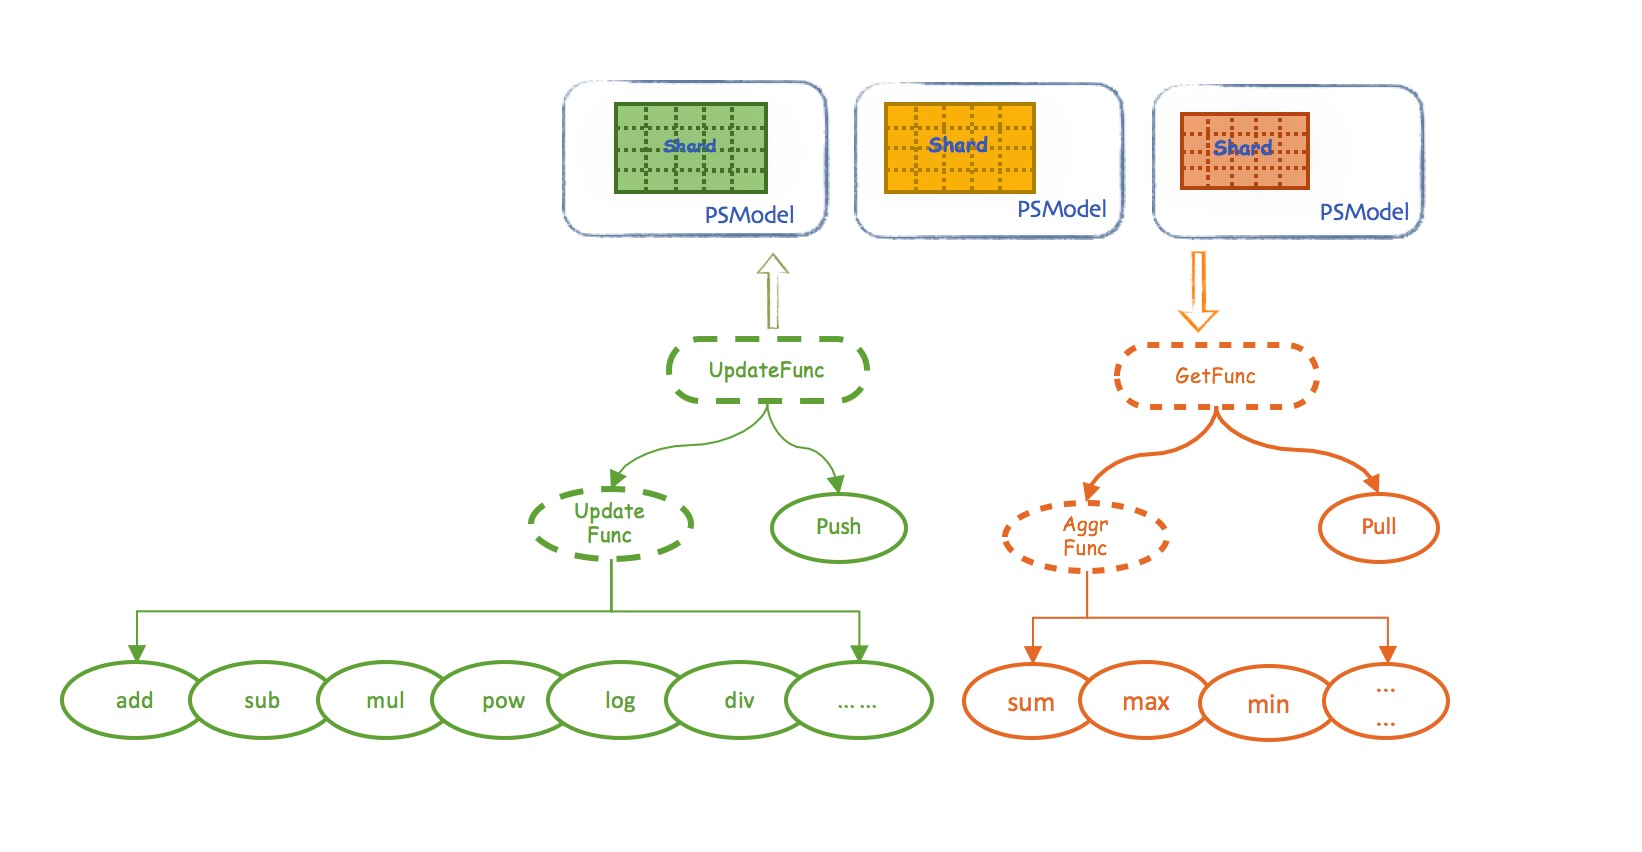
\includegraphics[keepaspectratio=true,width=\dimmin{}{\dimwidth{0.90}}]{images/angel_psFunc}{}\mdline{51}%mdk%mdk

%mdk-data-line={53}
\item{}
%mdk-data-line={53}
\mdline{53}GetFunc(参数获取)%mdk

%mdk-data-line={55}
\mdline{55}请求划分:操作的是整个模型参数,进行请求划分,生成一个请求列表,这个请求列表中,每一个请求都和一个模型参数分区对应%mdk

%mdk-data-line={57}
\mdline{57}请求发送:将请求列表中的所有请求,发送给模型参数分区所在的PSServer,PSServer以模型参数分区为单位执行参数获取和更新操作,并返回相应的结果%mdk

%mdk-data-line={59}
\mdline{59}请求合并:合并所有的模型分区级结果,得到最终的结果并返回%mdk%mdk

%mdk-data-line={61}
\item{}
%mdk-data-line={61}
\mdline{61}UpdateFunc(参数更新)%mdk

%mdk-data-line={63}
\mdline{63}请求划分:PSClient进行请求划分,生成一个请求列表,这个请求列表中的每一个请求都和一个模型参数分区对应%mdk

%mdk-data-line={65}
\mdline{65}请求发送:将请求列表中的所有请求发送给模型参数分区所在的PS实例,PS实例以模型参数分区为单位执行更新操作%mdk

%mdk-data-line={67}
\mdline{67}等待完成:等待所有请求完成后返回%mdk

%mdk-data-line={69}
%mdk-data-line={70}
\noindent\mdline{70}\textbf{Note}.
\mdline{71}无论是Get还是Update,具体的这3个阶段,其过程都是可以自定义的,从而实现千变万化的psFunc。%mdk%mdk%mdk
%mdk
\end{itemize}%mdk

%mdk-data-line={77}
\begin{mddefinitions}%mdk

\mddefterm{\noindent{\bfseries自定义模型切片}}%mdk

%mdk-data-line={77}
\begin{mdbmarginx}{}{}{}{1.5em}%mdk
\begin{mddefdata}%mdk
\mdline{77}Angel默认的模型分区:将模型切分成大小相等的矩形区域。1)尽量将一个模型平均分配到所有PS节点上;2)对于非常小的模型,将它们尽量放在一个PS节点上;3)对于多行的模型,尽量将同一行放在一个PS节点上
%mdk
\end{mddefdata}%mdk
\end{mdbmarginx}%mdk

%mdk-data-line={79}
\begin{mdbmarginx}{}{}{}{1.5em}%mdk
\begin{mddefdata}%mdk
\mdline{79}也可以自定义的记的模型分区:设置自定义的Partitioner,实现两个接口getPartitions和assignPartToServer,最后将其将其注入到PSModel的MatrixContext之中即可使用
%mdk
\end{mddefdata}%mdk
\end{mdbmarginx}%mdk

\mddefterm{\noindent{\bfseries支持多种容错}}%mdk

%mdk-data-line={80}
\begin{mdbmarginx}{}{}{}{1.5em}%mdk
\begin{mddefdata}%mdk
\mdline{80}PS容错采用了checkpoint的模式
%mdk
\end{mddefdata}%mdk
\end{mdbmarginx}%mdk

%mdk-data-line={82}
\begin{mdbmarginx}{}{}{}{1.5em}%mdk
\begin{mddefdata}%mdk
\mdline{82}挂掉的Worker实例可以从Master处获取当前迭代轮数等状态信息,从PS处获取最新模型参数,然后重新开始被断掉的迭代
%mdk
\end{mddefdata}%mdk
\end{mdbmarginx}%mdk

%mdk-data-line={83}
\begin{mdbmarginx}{}{}{}{1.5em}%mdk
\begin{mddefdata}%mdk
\mdline{83}Master定期将任务状态写入hdfs,挂掉后Yarn会重新拉起一个Angel的Master,加载状态信息,重新启动Worker和PS,从断点处重新开始计算。%mdk
\end{mddefdata}%mdk
\end{mdbmarginx}%mdk
%mdk
\end{mddefinitions}%mdk

%mdk-data-line={85}
\section{\mdline{85}4.\hspace*{0.5em}\mdline{85}Angel编译和运行}\label{sec-angel}%mdk%mdk

%mdk-data-line={87}
\begin{itemize}[noitemsep,topsep=\mdcompacttopsep]%mdk

%mdk-data-line={87}
\item\mdline{87}环境要求:Jdk \mdline{87}\textgreater{}\mdline{87}= 1.8 Maven \mdline{87}\textgreater{}\mdline{87}= 3.0.5 Protobuf \mdline{87}\textgreater{}\mdline{87}= 2.5.0且和Hadoop的Protobuf版本一致%mdk

%mdk-data-line={88}
\item\mdline{88}源码下载:git clone https://github.com/Tencent/angel%mdk

%mdk-data-line={89}
\item\mdline{89}编译:mvn clean package\mdline{89} \mdline{89}-Dmaven.test.skip=true  发布包位于dist/target目录下%mdk

%mdk-data-line={90}
\item\mdline{90}运行时可以选择本地运行,或通过Yarn提交到集群运行%mdk
%mdk
\end{itemize}%mdk

%mdk-data-line={93}
\section{\mdline{93}5.\hspace*{0.5em}\mdline{93}开发新算法过程}\label{section}%mdk%mdk

%mdk-data-line={95}
\begin{enumerate}[noitemsep,topsep=\mdcompacttopsep]%mdk

%mdk-data-line={95}
\item\mdline{95}定义一个模型,继承MLModel,里面定义参数模型及其他的一些配置%mdk

%mdk-data-line={96}
\item\mdline{96}定义一个Task,继承自TrainTask,定义模型的训练过程,需要实现parse()和train()两个方法,分别为解析数据和训练%mdk

%mdk-data-line={97}
\item\mdline{97}定义一个Runner,继承自MLRunner,用于将任务提交到集群,实现train()和predict()两个方法%mdk
%mdk
\end{enumerate}%mdk

%mdk-data-line={99}
\section{\mdline{99}6.\hspace*{0.5em}\mdline{99}总结}\label{section}%mdk%mdk

%mdk-data-line={100}
\noindent\mdline{100}通过默认的模型分区策略,和自定义的模型分区策略,Angel的模型分区上,在方便性和灵活性,做出了很好的平衡,为用户实现高效的复杂算法,打下了良好的基础。%mdk

%mdk-data-line={102}
\mdline{102}Angel实现了灵活多变的异步控制模式,为用户的算法,提供了最大化的便利,也解决了在大规模机器学习中,由于个别机器故障,引起严重的性能问题。%mdk

%mdk-data-line={104}
\mdline{104}随着psFunc的引入,模型的计算,也会发生在PSServer端。PSServer也将有一定的模型计算职责,而不是单纯的模型存储功能。合理的设计psFunc,将大大的加速算法的运行。
伴随着psFunc的引入和强化,在很多复杂的算法实现中,大大的降低了Worker要把模型完整的拖回来进行整体计算的可能性,从而曲线的实现了模型并行。%mdk%mdk


\end{document}
